%! Author = chaorn
%! Date = 06.09.24
\subsection{Verwendete Fuzzer}\label{subsec:verwendete-fuzzer}
In diesem Kapitel werden die in dieser Arbeit verwendeten Fuzzer vorgestellt.
Die Fuzzer \gls{afl}Net, boofuzz und Pulsar werden im Kontext der Performance-Analyse von Netzwerkfuzzern
verwendet und auf ihre Effektivität bei der Identifizierung von Schwachstellen in Netzwerkprotokollen untersucht.
Die Fuzzer boofuzz und \gls{afl}Net wurden in dieser Arbeit ausgewählt, da sie weit verbreitete Fuzzer mit umfangreicher
Dokumentation sind.
Pulsar wurde aufgrund seiner einzigartigen Fähigkeit, Netzwerkprotokolle zu erlernen und zu simulieren, ausgewählt.
Die Auswahl der drei Fuzzer ermöglicht es, verschiedene Ansätze und Techniken des Netzwerkfuzzings zu vergleichen und
einen möglichst umfassenden Einblick in die Herangehensweisen der Fuzzer zu erhalten.
\subsubsection{AFLNet}\label{subsubsec:aflnet}
\gls{afl} ist ein Fuzzer, der auf dem Prinzip der Codeabdeckung basiert.
Er zählt somit zu der Familie der Grey-Box Fuzzer und basiert auf einer mutationsbasierten Fuzzing-Technik.
Bei \gls{afl} handelt es sich ebenso um einen Applikationsfuzzer, welcher mithilfe eines Eingabestreams Daten
an ein \gls{zup} sendet und somit die Software auf Schwachstellen testet.\newline
Zur Analyse des Programms wird in dieser Arbeit jedoch ein Derivat von \gls{afl}(\gls{afl}Net) verwendet.
Es unterscheidet sich von dem ursprünglichen \gls{afl} dadurch, dass es speziell für die Analyse von Netzwerkprotokollen
entwickelt wurde.
Die Kernfunktionalität von \gls{afl} bleibt jedoch erhalten und wird um die Möglichkeit erweitert, Netzwerkprotokolle zu
analysieren.\newline
Hierzu müssen die Netzwerkpakete, die an das \gls{zup} gesendet werden, in einem speziellen Format vorliegen.
Die Extraktion der Netzwerkpakete erfolgt mithilfe eines \gls{pcap}-Dump-Files.
Diese Dump-Files enthalten den Netzwerkverkehr, der zwischen zwei Kommunikationspartnern stattgefunden hat.
Um diese Dump-Files zu generieren und somit den Netzwerkverkehr aufzunehmen wird das Tool \texttt{tcpdump} verwendet.
Zur Generierung der Netzwerkpakete wird das \gls{pcap}-Dump-File in ein \gls{afl}-kompatibles Format umgewandelt, indem
die rohen Datenflüsse extrahiert und in eine Datei geschrieben werden.
Die Extraktion der Datenflüsse kann mit Netzwerkanalyse-Tools wie \texttt{Wireshark} oder \texttt{tcpdump} erfolgen.
Hierzu wird im Repository von \gls{afl}Net~\cite{aflnet-repo} bereits eine Herangehensweise vorgestellt, wie die Datenflüsse mit
Wireshark extrahiert werden können.
Diese Datenflüsse werden dann als Bytestream von \gls{afl} als Eingabe verwendet, um das \gls{zup} zu fuzzen.
\begin{figure}[H]
    \centering
    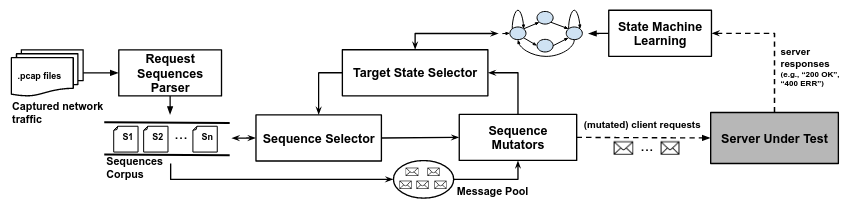
\includegraphics[width=\textwidth]{img/aflnet_arch}
    \caption[Architektur des AFLNet Fuzzers]{Die Abbildung zeigt die Architektur von \gls{afl}Net nach Pham Van-Thuan~\cite{AFLNet}.}
    \label{fig:aflnet_architecture}
\end{figure}
\noindent Zuerst muss das \gls{zup} gestartet und mir Eingaben gefüttert werden.
Während der Transaktion der Nachrichten wird der einhergehende Traffic mit einem Aufnahmeprogramm wie \texttt{tcpdump} aufgezeichnet.
Die aufgezeichneten Daten werden in ein \gls{pcap}-Dump-File geschrieben und müssen anschließend analysiert werden.
Dabei muss der Netzwerkverkehr in ein Format umgewandelt werden, das von \gls{afl}Net verstanden wird.
Dieses Format besteht in dem Fall dieser Arbeit aus einem Bytestream, der die Nachrichten des Netzwerkverkehrs enthält.
Die Nachrichten werden in einer Datei abgelegt und können dann von \gls{afl}Net als Eingabe verwendet werden.
Besonderes Augenmerk hierbei liegt auf der Analyse des Netzwerkverkehrs und der daraus resultierenden State Machine.
\gls{afl}Net analysiert den Netzwerkverkehr und extrahiert die Nachrichten, die zwischen Client und Server ausgetauscht werden.
Werden bei der Ausführung von Nachrichten bestimmte Zustände erreicht, so werden diese Zustände in einer State Machine
abgebildet und die State Machine mit dem neuen Zustand als Node erweitert.
Die State Machine wird mithilfe von \gls{afl}Net erlernt und ermöglicht es, den Zustand des \gls{zup} nachzuverfolgen.
Das Erlernen der State Machine erfolgt durch das Aufstellen eines Graphen, der die Zustände des \gls{zup} abbildet.
Hierbei werden die Zustände basierend auf den gesendeten Nachrichten und den vom \gls{zup} generierten Antworten identifiziert.
Dieser Graph wird initial bei der Testphase der Nachrichten erstellt und bei jeder neuen Nachricht erweitert.
Die Erweiterung des Graphen erfolgt durch das Hinzufügen von neuen Zuständen, die durch die Nachrichten erreicht werden~\cite{AFLNet}.
\newline
Anschließend werden die Nachrichten mit den enthaltenen Nachrichtensequenzen an einen in \gls{afl}Net implementierten
Sequence-Mutator übergeben.
Dieser Mutator generiert aus den gesendeten Nachrichten neue mutierte Nachrichten, die an das \gls{zup} übergeben werden
können.
\subsubsection{Boofuzz}\label{subsubsec:boofuzz}
Boofuzz ist ein Open-Source-Fuzzing-Framework, das zur automatisierten Sicherheitsprüfung von Software verwendet wird.
Es wurde als Fork des populären Sulley Fuzzing Frameworks entwickelt und bietet verbesserte Stabilität, erweiterte Funktionen
und aktive Wartung.
Boofuzz ist in Python geschrieben und ermöglicht das Erstellen von Fuzzing-Kampagnen durch die Definition von Testfällen,
die systematisch verschiedene Protokollfelder und Eingabeparameter abdecken.
Das Framework unterstützt sowohl Netzwerkprotokolle als auch dateibasierte Anwendungen, was es vielseitig einsetzbar macht.
Dabei kann es beispielsweise Protokolle wie HTTP, FTP oder Telnet fuzzen, um Schwachstellen in Netzwerkdiensten zu identifizieren.
Ein zentrales Merkmal von boofuzz ist seine Fähigkeit zur Überwachung des Zustands des Zielsystems während des Fuzzings.
Hierbei handelt es sich jedoch nicht um \textit{state-awareness} -- also den tatsächlich erreichten Zustand eines Programms --
sondern ob ein Dienst abgestürzt ist, und entsprechend reagieren, indem es den Testprozess anpasst oder erneut startet.
Da keine Informationen über den internen Zustand des Zielsystems benötigt werden und die Generierung der Eingaben
willkürlicher Natur ist, handelt es sich bei boofuzz um einen \textit{"Brute Force"} Black-Box-Fuzzer.
\subsubsection{Pulsar}\label{subsubsec:pulsar}
Pulsar ist ein Fuzzer und wird zu der Familie der Black-Box-Fuzzer gezählt.
Der Fuzzer wird dafür verwendet, um Internet Protokolle zu testen.
Er ermöglicht es, ohne jedweden Quellcode anhand von gesammelten Traffic-Dumps eine State Machine eines \gls{zup} zu erlernen.
Das Besondere an diesem Fuzzer ist, dass er anhand von gesammelten Daten ein Model trainiert,
welches es dem Untersucher des Programmes ermöglicht, das Programm zu simulieren und schlussendlich
gezielt zu fuzzen.
Bei der Simulation des Protokolls kann der Fuzzer sowohl die Rolle des Clients, als auch die Roller
des Servers einnehmen.
Gerade dieser Punkt ermöglicht es dem Untersucher des Programms große Flexibilität bei der Untersuchung zu erreichen.
Somit kann ein großer Teil des Programms untersucht werden und möglichst tief in die Struktur des \gls{zup} eingegriffen werden.
\newline
\noindent Das Training des Modells beruht auf der Analyse des eingefangenen Netzwerkverkehrs.
Dabei werden verschiedene Nachrichten von sowohl Client- als auch Serverseite auf Byte-Ebene untersucht und
ähnliche Strukturen extrahiert.
Die daraus extrahierten Nachrichtensequenzen werden darauffolgend in einen endlich-deterministischen Vektor abgebildet.
Die Zusammenkunft aus mehreren Vektoren ergibt ein Cluster.
Anhand der entstandenen Cluster wird eine approximierte Abbildung der State-Machine des Protokolls geschlussfolgert.
Bei der Erschließung der State Machine können die tatsächlichen Zustände nur teilweise erschlossen werden und ist somit
von der Güte des gesammelten Netzwerkverkehrs abhängig.
Der Netzwerkverkehr wird bei der Untersuchung von Pulsar annotiert, um die Nachrichten von Client und Server unterscheiden
zu können.
Zusammenhänge zwischen den Nachrichten werden anhand von bereits beobachteten Nachrichten erschlossen.
Diese werden in Tupeln miteinander verglichen und miteinander assoziiert.
Nachdem die Assoziation aller Mitteilungen abgeschlossen ist, besteht ein Markov Modell zweiter Ordnung.
Dieses Modell wird in einem Graphen abgebildet und kann somit als eine Annäherung der State Machine interpretiert werden.
Das Markov Modell wird im anschluss mit einem \gls{dfa} minimiert.
Der dabei entstandene \gls{dfa} erlaubt es Analysten die Zustände manuell untersuchen zu können und gegebenenfalls
die Zustände zu verfeinern und nachzuvollziehen~\cite{pulsar}.